% !TEX root = handbook-physics.tex
%!TEX TS-program = xelatex
%!TEX encoding = UTF-8 Unicode


\chapter{Kinematics}
\label{ch-01}

\section{Mechanical Motion. The Subject Matter of Mechanics}
\label{sec-1.1}
\subsection{}\label{1.1.1} The simplest form of motion in nature is \emph{mechanical motion}. It consists of changes in the relative positions of bodies or their parts in space in the course of time. The branch of phys­ics dealing with the laws of mechanical motion is called \emph{me­chanics}. In a more narrow sense of the word, this is often under­ stood to mean \emph{classical mechanics}, which deals with the motion of macroscopic bodies travelling at velocities a great many times less than that of light in free space. Classical mechanics is based on Newton’s laws and is therefore frequently referred to as \emph{Newtonian mechanics}. The laws of motion of bodies at velocities close to that of light in free space are taken up in \emph{relativistic mechanics} (\ref{5.1.1}), and the laws of motion of micro­ particles (for example, the electrons in atoms, molecules, crystals, etc.) are the subject matter of \emph{quantum mechanics} (\ref{38.1.1}). 

\subsection{}\label{1.1.2}Classical mechanics comprises three basic branches: sta­tics, kinematics and dynamics. Statics deals with the laws for the composition of forces and the conditions for the equilibrium of bodies. \emph{Kinematics} provides a mathematical description of all possible kinds of mechanical motion, regardless of what causes each particular kind of motion. \emph{Dynamics} investigates the effect of the interaction between bodies on their mechanical motion. 

\subsection{}\label{1.1.3}The mechanical properties of bodies are determined by their chemical nature, internal structure and state. These are beyond the scope of mechanics and are studied in other branches of physics. Hence, in accordance with the conditions of each specific problem on hand, various simplified models are employed to describe real bodies in motion. These include the particle, the perfectly rigid body, the perfectly elastic body, the perfectly inelastic body and others.

A \emph{material point}, or \emph{particle}, is a body whose shape and size are of no consequence under the conditions of the problem being considered. For example, in a first approximation, the motion of a ship from one point to another can be dealt with as the motion of a particle. If, however, it becomes necessary to take into account such details of this motion as the pitching and rolling of the ship by swells or heavy seas, the ship should be dealt with as an extended body of definite shape. In the liter­ature the word particle is more frequently used than mate­rial point.

Any extended body or system of such bodies, making up the \emph{mechanical system} being investigated, can be regarded as a \emph{system of particles}. For this purpose, ail the bodies of the system can be conceived of as being broken down into such a large number of parts that the size of each part is negligibly small compared to the sizes of the bodies themselves.

\subsection{}\label{1.1.4} A \emph{perfectly rigid body}, or simply \emph{rigid body}, is one whose deformation can be neglected under the conditions of the given problem. The distance between any two points of a rigid body remains constant no matter what action the body is subjected to. A perfectly rigid body can be regarded as a system of par­ticles rigidly connected to one another.

A \emph{perfectly elastic body} is one whose deformation obeys Hooke’s law (\ref{40.3.4}). After the external forces applied to such a body have been removed, its initial size and shape are completely restored.

A \emph{perfectly inelastic body} is one that completely retains its deformed state, caused by external forces applied to the body, when these forces have been removed.

\section[Frames of Reference. Path, Path Length]{Frames of Reference. Path, Path Length and Displacement Vector of a Particle}
\label{sec-1.2}

\subsection{}\label{1.2.1} The position of a body in space can be specified only in reference to other bodies. It makes sense, for instance, to speak of the location of the planets with respect to the sun, that of an air liner or steamship with respect to the earth, but we cannot indicate their position in space ``in general'' without ref­erence to some specific body. A perfectly rigid body in which a coordinate system is rigidly fixed, furnished with a ``clock'' and employed to determine the position of bodies and particles being investigated in space at various instants of time, is called a frame of reference. Sometimes the frame of reference is the coordinate system itself if it is provided with a ``clock'' and the solid in which the system is rigidly fixed is called the body of reference. In each specific problem the frame of refer­ence is selected so as to simplify the problem to the maximum extent. Inertial frames of reference (\ref{2.1.2}) are the most com­monly used in physics.

\subsection{}\label{1.2.2} Most extensively employed is the Cartesian rectangular system of coordinates (\figr{fig-01-01}) whose orthonormal (normal orthogonal) basis is formed by the three vectors $\vb{i}$, $\vb{j}$ and $\vb{k}$, which  are unit vectors with respect to their magnitudes, mutually orthogonal and pass through the origin $O$ of coordinates. The position of an arbitrary point $M$ is specified by the radius vector $\vb{r}$, which connects the ori­gin $O$ of coordinates to point $M$. Vector $\vb{r}$ can be resolved along the axes $\vb{i}$, $\vb{j}$ and $\vb{k}$ of the basis as follows:
\begin{equation*}%
\vb{r}= x \vb{i} + y \vb{j} + z \vb{k}
\end{equation*}
where $x\vb{i}$, $y\vb{j}$ and $z\vb{k}$ are the com­ponents of vector $\vb{r}$ along the coordinate axes. The coefficients of resolution, $x$, $y$ and $z$, are the Cartesian coordinates of point $M$ and, due to the orthogo­nality of the vectors of the basis, the projections of radius vector $\vb{r}$ on the corresponding coordinate axes.

\begin{wrapfigure}{r}{0.5\linewidth}
\centering
%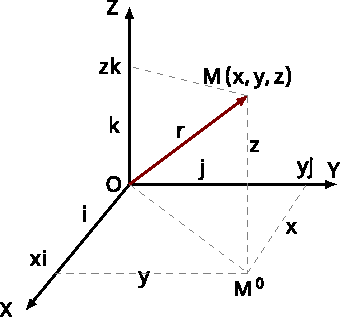
\includegraphics{figs/ch-01/fig-01-01.pdf}
% !TEX root = ../../handbook-physics.tex
%!TEX TS-program = pdflatex
%!TEX encoding = UTF-8 Unicode


%\documentclass{article}
%\usepackage[svgnames]{xcolor}
%\usepackage{tikz}
%\usepackage{amsmath}
%\usepackage{physics}
%
%\begin{document}
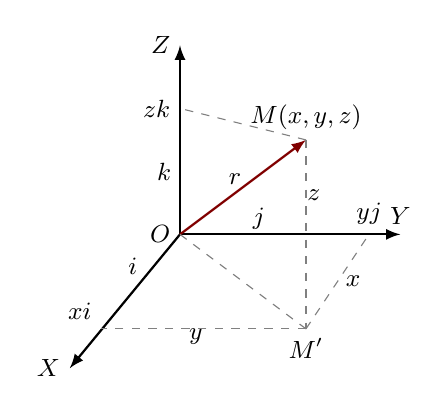
\begin{tikzpicture}[scale=0.4,font=\small]
		\node [] (0) at (0, 6){};
		\node [] (1) at (0, 0) {};
		\node [] (2) at (-3.5, -4.25) {};
		\node [] (3) at (7, 0) {};
		\node [] (4) at (4, 3) {};
		\node [] (5) at (4, -3) {};
		\node [] (6) at (0, 4) {};
		\node [] (7) at (6, 0) {};
		\node [] (8) at (-2.5, -3) {};
		\node [] (9) at (1.75, 1.75) {};
		\node [] (10) at (1.75, 1.75) {$\vb{r}$};
		\node [] (11) at (-0.5, 2) {$\vb{k}$};
		\node [] (12) at (-1.5, -1) {$\vb{i}$};
		\node [] (13) at (2.5, 0.5) {$\vb{j}$};
		\node [] (14) at (0.5, -3.25) {};
		\node [] (15) at (5.5, -1.5) {};
		\node [] (16) at (4.25, 1.25) {};
		\node [] (18) at (5.5, -1.5) {$x$};
		\node [] (19) at (0.5, -3.25) {};
		\node [] (20) at (0.5, -3.25) {$y$};
		\node [] (21) at (4.25, 1.25) {$z$};
		\draw [thick,latex-](0.center) to (1.center);
		\draw [thick,-latex](1.center) to (2.center);
		\draw [thick,-latex](1.center) to (3.center);
		\draw [thick,-latex,Maroon](1.center) to (4.center);
		\draw [dashed,gray](1.center) to (5.center);
		\draw [dashed,gray](4.center) to (6.center);
		\draw [dashed,gray](4.center) to (5.center);
		\draw [dashed,gray](5.center) to (7.center);
		\draw [dashed,gray](5.center) to (8.center);
		\node [left] at (0,0) {$O$};
		\node [left] at (0,6) {$Z$};
		\node [left] at (-3.5, -4.25) {$X$};
		\node [above] at (7, 0) {$Y$};
		\node [above] at (4, 3) {$M (x,y,z)$};
		\node [below] at (4, -3) {$M'$};
		\node [left] at (0,4) {$z\vb{k}$};
		\node [above] at (6,0) {$y\vb{j}$};
		\node [above left] at (-2.5, -3) {$x\vb{i}$};
\end{tikzpicture}
%\end{document}
%  \vspace{-13pt}
\caption{Cartesian system of coordinates.}
\label{fig-01-01}
\end{wrapfigure}

The motion of a particle is completely specified if three continuous and single-valued functions of the time $t$,
\begin{equation*}%
x= x(t), \,\,y= y(t)\,\,\textrm{and}\,\, z= z(t),
\end{equation*}
are given to describe the changes in the coordinates of the particle with time.


These equations are said to be the \emph{kinematic equations of motion of a particle}. They are equivalent to the single vector equation
$\vb{r} = \vb{r} (t)$, for a moving particle.

\subsection{}\label{1.2.3} The line described by a moving particle in space is called its \emph{path}. The kinematic equations of motion of a particle spec­ify the equation of its path in parametric form (the parameter being the time $t$). Depending upon the shape of the path, distinction is made between \emph{rectilinear} and \emph{curvilinear} motion. The motion of a particle is said to be \emph{plane} if its path lies com­pletely in a single plane.

The mechanical motion of a body is relative, i.e. the nature of the motion and, in particular, the kind of path travelled by the points of the body depend upon the chosen frame of re­ference.

\subsection{}\label{1.2.4} In the general case, the path of a moving particle is a spatial, rather than plane, curve. Introduced for such curves is the concept of an \emph{osculating plane}. The osculating plane at the arbitrary point $M$ of a curve is in the limiting position of a plane passing through any three points of the curve when these points approach point $M$ without limit.

An \emph{osculating circle} at point $M$ of a curve is the limit of a circle passing through three points of the curve being considered when these points approach po­int $M$ without limit. The oscu­lating circle lies in the oscula­ting plane. The centre of the osculating circle and its radius are called the \emph{centre of curvature} and \emph{radius of curvature}, at point $M$, of the curve being considered. The straight line connecting point $M$ to the centre of curvature is called the \emph{principal normal} to the curve at point $M$. The tan­gent to the curve at point $M$ is perpendicular to the principal normal and also lies in the osculating plane.

\subsection{}\label{1.2.5} The \emph{path length} is the sum of the lengths of all the por­tions of the path over which the particle passes m the given interval of time. The instant of time $t = t_{0}$, from which we begin to consider the motion of a particle, is called the initial instant of time, and the position of the particle at this instant (point $A$ in \figr{fig-01-02}) is called its initial position. Owing to the arbitrary nature of the time reference point it is usually as­sumed that $t_{0}= 0$. 

\begin{wrapfigure}{l}{0.5\linewidth}
\centering
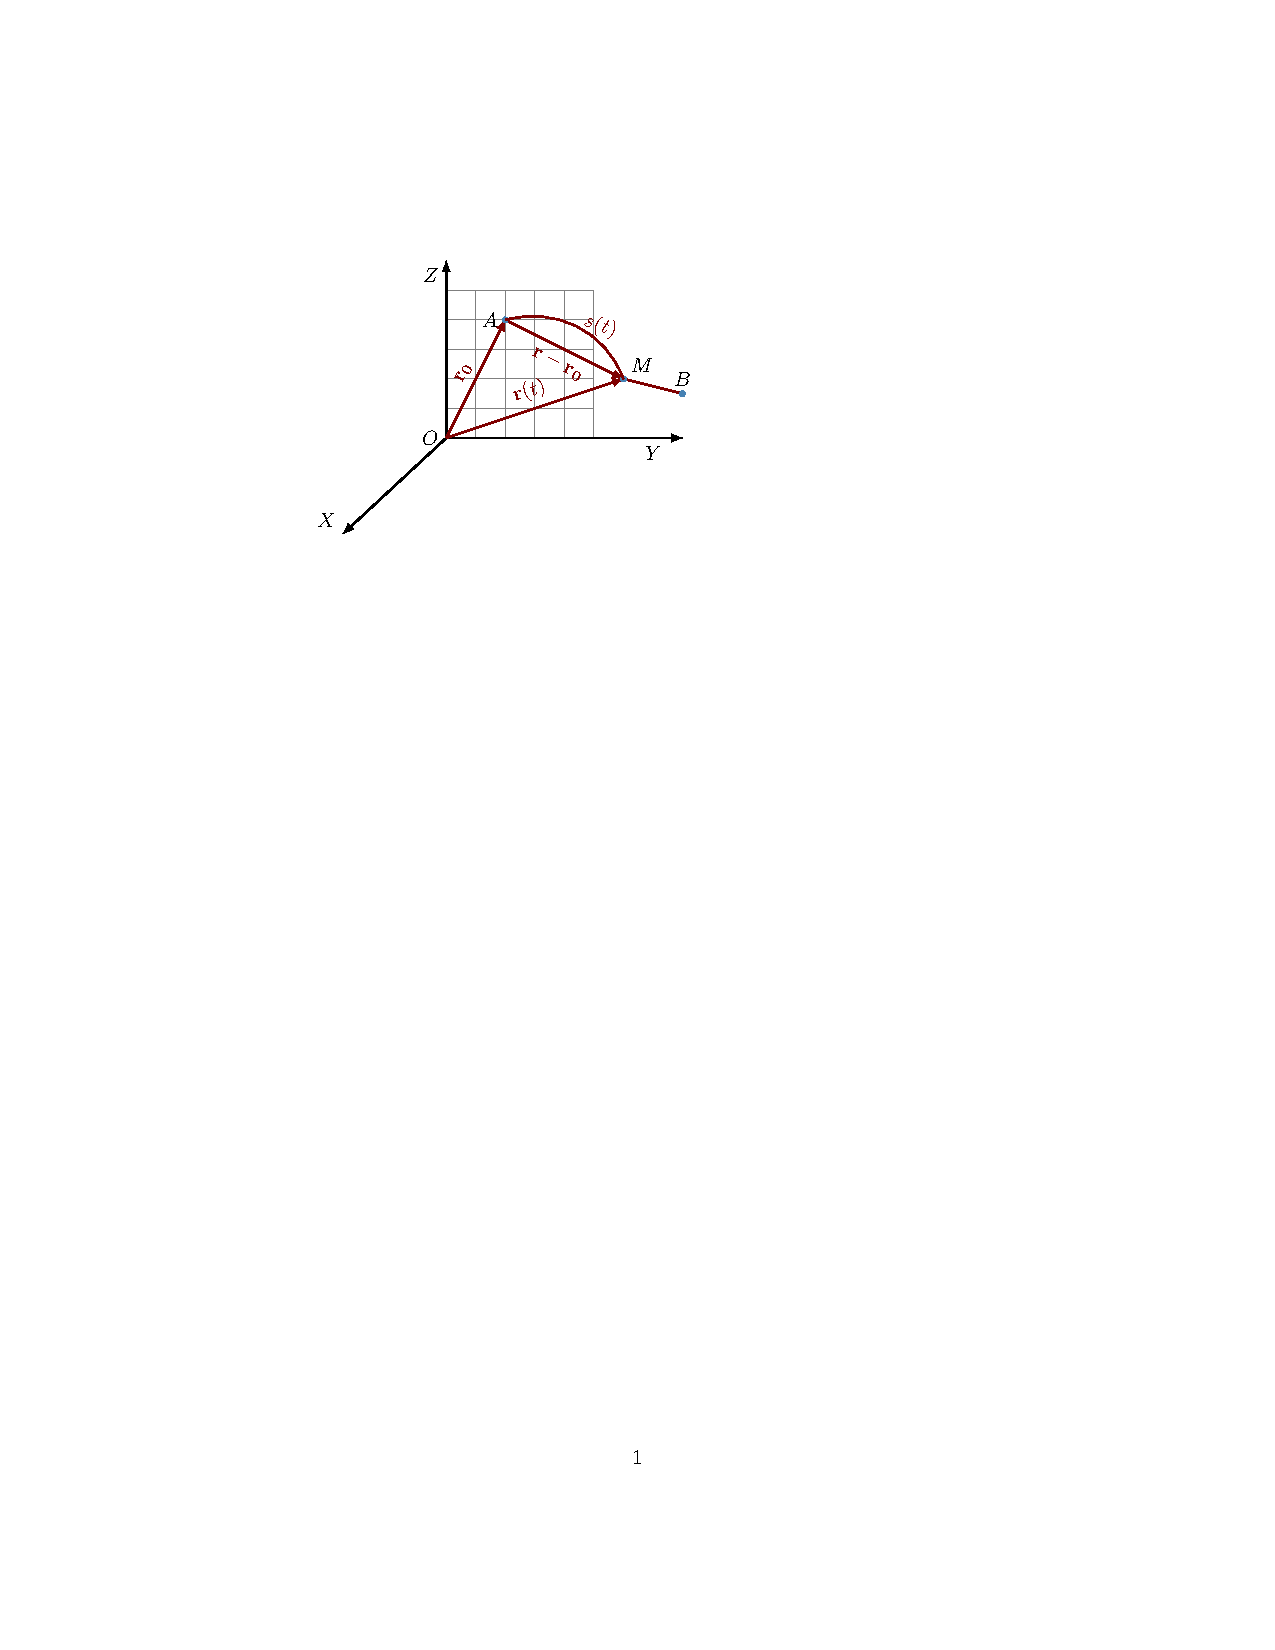
\includegraphics{figs/ch-01/fig-01-02.pdf}
\caption{A particle moving on a curve.}
\label{fig-01-02}
\end{wrapfigure}

The path length $s$, travelled by the particle from its initial position, is a scalar function of time: $s = s (t)$. As is obvious from its definition, the path length of a particle cannot be a negative quantity. If the particle travels along an arc of the path $AB$ (\figr{fig-01-02}), always in the same direction and is at point $M$ at the instant of time $t$,then $s(t)= \widearc{AM}$. If the particle travels along the path in a more complicated way, for example if it travels from $A$ to $B$, reaching $B$ at the instant of time $t_{1}< t$, and then reverses, returning to point $M$ at instant $t$, then $s (t) = \widearc{AB} + \widearc{BM}$.


\subsection{}\label{1.2.6} The displacement vector of a moving particle during the time interval from $t= t_{1}$ to $t= t_{2}$ is the vector from the, position of the particle at the instant of time $t_{1}$ to its position at instant $t_{2}$. It is equal to the increment in the radius vector of the particle during the time interval being considered:
\begin{equation*}%
\vb{r_{2}} - \vb{r_{1}} = \vb{r}(t_{2}) - \vb{r}t_{1}
\end{equation*}
The displacement vector is always directed along the chord subtending the corresponding portion of the path.

Shown in \figr{fig-01-02} is the displacement vector of the particle for the time interval from $t_{0}$ to $t$. It is equal to $\vb{r}- \vb{r_{0}} = \vb{r} (t)- \vb{r}(t_{0})$.

The displacement vector of a moving particle for the time inter­val from $t$ to $t + \Delta t$ equals
\begin{equation*}%
\Delta r = r (t + \Delta t) - r (t) = \Delta x \times \vb{i} + \Delta y \times \vb{j} + \Delta z \times \vb{k}
\end{equation*}
where $\Delta x$, $\Delta y$ and $\Delta z$ are the increments (changes) in the coordi­nates of the particle during the time interval being considered. 

\subsection{}\label{1.2.7} A particle travelling freely in space can accomplish only three \emph{independent motions}, i.e. motions that cannot be repre­sented as combinations of the other two. As a matter of fact, the motion of a particle along each of the axes of a Cartesian rectangular coordinate system cannot be obtained by its motion along the other two axes. The number of independent motions that a mechanical system can accomplish is called the \emph{number of degrees of freedom} of the system. Hence, a free particle has three degrees of freedom.
